\section{Exit pressure study}
Solver Parameters:
\begin{description}[noitemsep]
    \item[Timestepping Scheme:] Euler Explicit
    \item[CFL:] 0.1
    \item[Spatial Scheme:] Scalar Dissipation
    \item[Grid Points:] 50
\end{description}
The value of $\epsilon$ has been tweaked for the $\pexit = 0.76$ case such only three points
are observed in the shock -- it was not possible to get better than this. Dissipation
is directly correlated to $\epsilon$: the lower the value, the lower the dissipation in the
scheme. Thus, a relatively low $\epsilon$ is needed in order to get a sharp shock. The
``best'' $\epsilon$ was determined to be 0.05.

Results are shown in~\Cref{fig:q2}. While none of the solutions blew up with the chosen
$\epsilon$, i.e. the code was stable for all \pexit, wiggles can be observed for
$\pexit = 0.72p_t, 0.68p_t$. This is interesting, since it seems that the low dissipation
for those solutions lead to dispersion errors becoming dominant!
\begin{figure}
    \centering
    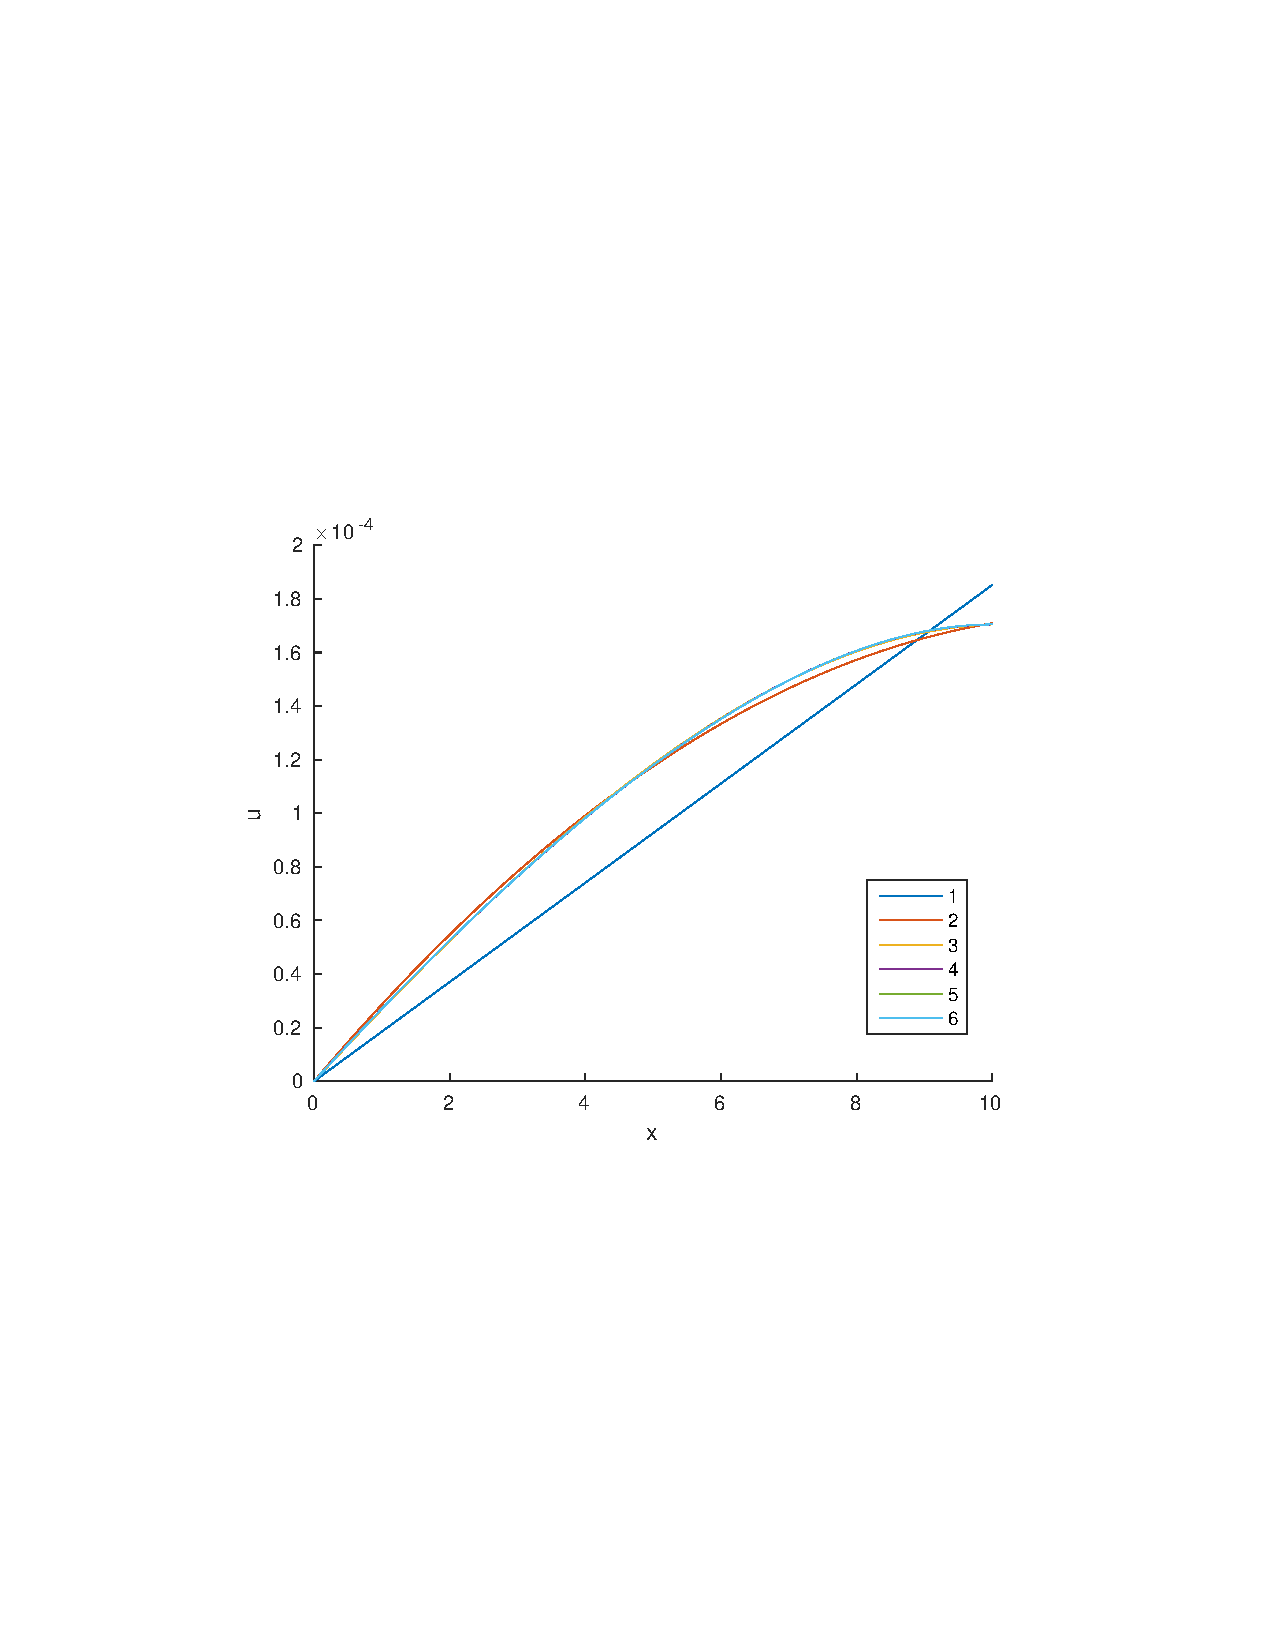
\includegraphics[width=0.9\textwidth]{./figs/q2}
    \caption{Solution for various \pexit with $\epsilon = 0.05$.}\label{fig:q2}
\end{figure}

Moreover, it can be seen that the $\pexit = 0.6p_t$ solution is fully supersonic, which
is not physically possible and is actually due to the lack of dissipation in the scheme.
This is shown in~\Cref{fig:q2_eps}. It can be seen that too low of an $\epsilon$ leads to
one of the following:
\begin{enumerate}
    \item The shock being pushed completely out of the exit and a supersonic solution
        ($\epsilon = 0.05$).
    \item A blow up in the solution ($\epsilon = 0.01$).
\end{enumerate}
On the other hand, too high of an epsilon ($\epsilon = 0.8$) results in an overly smoothed
shock. Thus, the value of $\epsilon$ should be chosen with care.

It should also be noted that the CFL value directly affects the range of
optimal (and allowable) $\epsilon$, since reducing the CFL increases dissipation
in the timestepping scheme. For instance, if the CFL were increased to 0.4, which would
decrease dissipation in timestepping, an $\epsilon$ of at least 0.2 would be necessary
for convergence.
\begin{figure}
    \centering
    \includegraphics[width=0.9\textwidth]{./figs/q2_eps}
    \caption{Results for $\pexit = 0.6p_t$ with various values of $\epsilon$.}
    \label{fig:q2_eps}
\end{figure}
